%% main.tex
%% Copyright 2022 skyleaworlder
%
% This work may be distributed and/or modified under the
% conditions of the LaTeX Project Public License, either version 1.3
% of this license or (at your option) any later version.
% The latest version of this license is in
%   http://www.latex-project.org/lppl.txt
% and version 1.3 or later is part of all distributions of LaTeX
% version 2003/12/01 or later.
%
% This work has the LPPL maintenance status "maintained".
%
% This Current Maintainer of this work is skyleaworlder.
%
% This work consists of all the *.tex and *.sty files in
%   https://github.com/TJ-CSCCG/Tongji-Beamer
\documentclass{ctexbeamer}

\usepackage{amsthm}
\usepackage{biblatex}
\addbibresource{reference.bib}
\setbeamertemplate{bibliography item}[text]

\usetheme{tongji}

%Information to be included in the title page:
\title[Visionary Art]{Visionary Art}
\subtitle{人工智能绘画分享站:项目开发里程碑1汇报}
\author[Software Engineering: Group 11]{
    2051857 曾诗容, \\
    2052636 陈骁, \\
    2050250 李其桐, \\
    2054080 林奕如, \\
    2053865 刘昱彤, \\
    1751118 吴达鹏, \\
    2053868 于采篱
}
\institute[CS Dept., CEIE, Tongji Univ.]{
    Computer Science and Technology Department, College of Electronic and Information Engineering(CEIE), Tongji University. \\
    同济大学\ 电子与信息工程学院\ 计算机科学与技术系\
}
\date{\today}

\begin{document}

\begin{frame}
    \titlepage
\end{frame}

%% introductioin.tex
%% Copyright 2022 skyleaworlder
%
% This work may be distributed and/or modified under the
% conditions of the LaTeX Project Public License, either version 1.3
% of this license or (at your option) any later version.
% The latest version of this license is in
%   http://www.latex-project.org/lppl.txt
% and version 1.3 or later is part of all distributions of LaTeX
% version 2003/12/01 or later.
%
% This work has the LPPL maintenance status "maintained".
%
% This Current Maintainer of this work is skyleaworlder.
%
% This work consists of all the *.tex and *.sty files in
%   https://github.com/TJ-CSCCG/Tongji-Beamer
\section{引言}
    \begin{frame}
    % “无序列表” 与 “有序列表” 使用
    \frametitle{引言}
        \footnotesize
        \begin{block}{项目提出背景}
            \begin{itemize}
                \item 	当前,ChatGPT已经发布并且对公众开放了服务接口,这无疑标志着一个人工智能的新纪元已然到来。通过ChatGPT的强势赋能,使得许多传统工作流都得到了极大的颠覆与创新,在达到更高效率的同时也能够确保质量。本项目正是在这一背景下,基于ChatGPT的公开API接口,搭建一个能够根据用户的自然语言描述需求,自动生成Markdown格式文档,然后通过Markdown解析器处理文件文本内容从而生成ppt的软件系统,从而能够在人们的实际文档设计与编写工作中,以一个可靠软件助手的姿态提供辅助,有效提升人们的工作效率。
            \end{itemize}
        \end{block}

        \begin{block}{项目意义}
            \begin{enumerate}
                \item 为响应在互联网传统工作方式中,企业内部、学生和个人对PPT文档的自动化生成和在线编辑需求而进行设计和开发。
                \item 为用户节省编辑成本,提升编辑效率,拥有广泛的应用前景。
                \item 对于其它竞品的相关功能特性进行研究分析,并且在其基础上进行精炼、完善,同时围绕核心业务设计并且实现额外的使用子功能模块。
            \end{enumerate}
        \end{block}
    \end{frame}


\section{本次里程碑任务}
\begin{frame}
    \frametitle{小组项目启动会工作项}
    \begin{itemize}
        \item 确定项目开发技术栈,搭建项目开发环境,使得相关框架能够正确集成并且运行。
        \item 根据甲方项目需求SRS文档,完成项目的需求分析,确定项目的主要功能,完成项目的功能设计与主要功能模块划分。
        \item 完成项目软件架构的逻辑设计和物理设计,主要包括数据库schema设计、索引设计、存储过程设计和视图设计,基于Restful API接口规范进行后端接口路由和功能设计等。
        \item 基于上述设计内容,使用华为云平台进行版本管理,将大功能模块设置为EPIC工作项,并且在Epic下抽取Feature,对于每个Feature进一步划分User Story,并且确定第一次迭代中需要实现的用户故事,最后分配工作到每位组员进行代码开发。
    \end{itemize}
\end{frame}

\begin{frame}
    \frametitle{工作项总览}
    我们小组在项目启动会中根据上述里程碑任务计划,详细讨论了项目的需求分析、软件架构设计、项目管理等内容,将设计细节落实到华为云工作项和开发文档,最终确定了本次里程碑任务的工作项,如下图所示:
        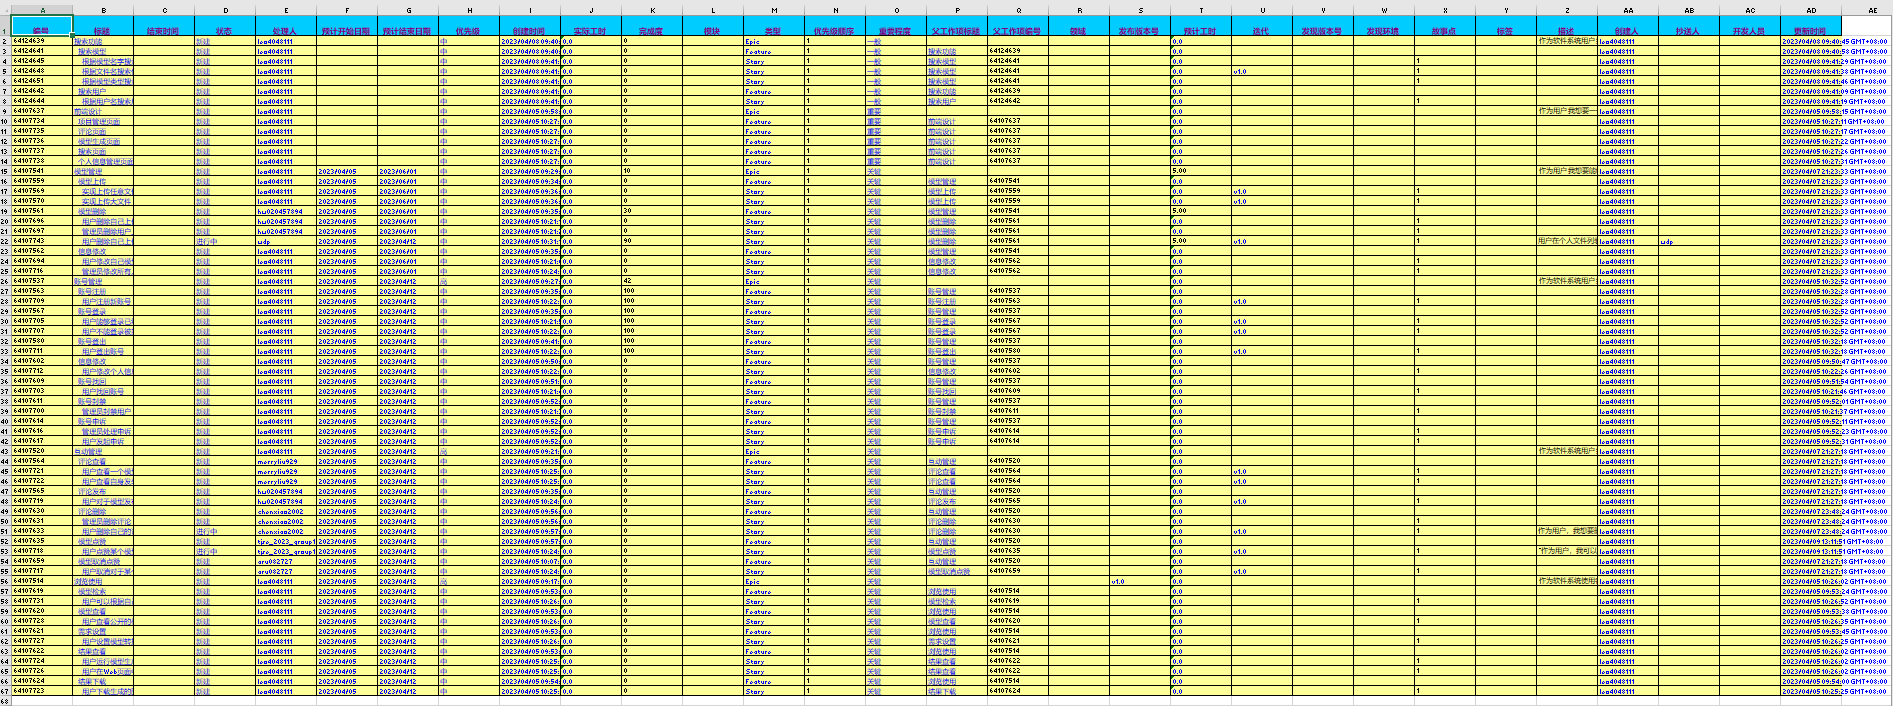
\includegraphics[width=2\textwidth]{contents/figure/work_items_overall.png}
\end{frame}

\begin{frame}
    \frametitle{项目技术栈}
    \begin{itemize}
        \item 主要开发语言:Python + HTML + CSS(SCSS) + JavaScript(Vue.js)
        \item HTTP服务器:Tornado
        \item 持久层框架:SQLAlchemy
        \item 数据库服务:MySQL + Redis
        \item 版本管理工具:Git
        \item 远程代码托管平台:华为云
        \item 接口管理与自动化测试工具:Apifox + Mock.js
    \end{itemize}
\end{frame}
\section{第一次迭代计划完成的用户故事}
\begin{frame}
    \frametitle{第一次迭代计划完成的用户故事}
    第一次迭代中,我们小组计划构建一个完整可用的软件系统架构,并且完成下列用户故事:
    \begin{figure}[H]
        \centering
        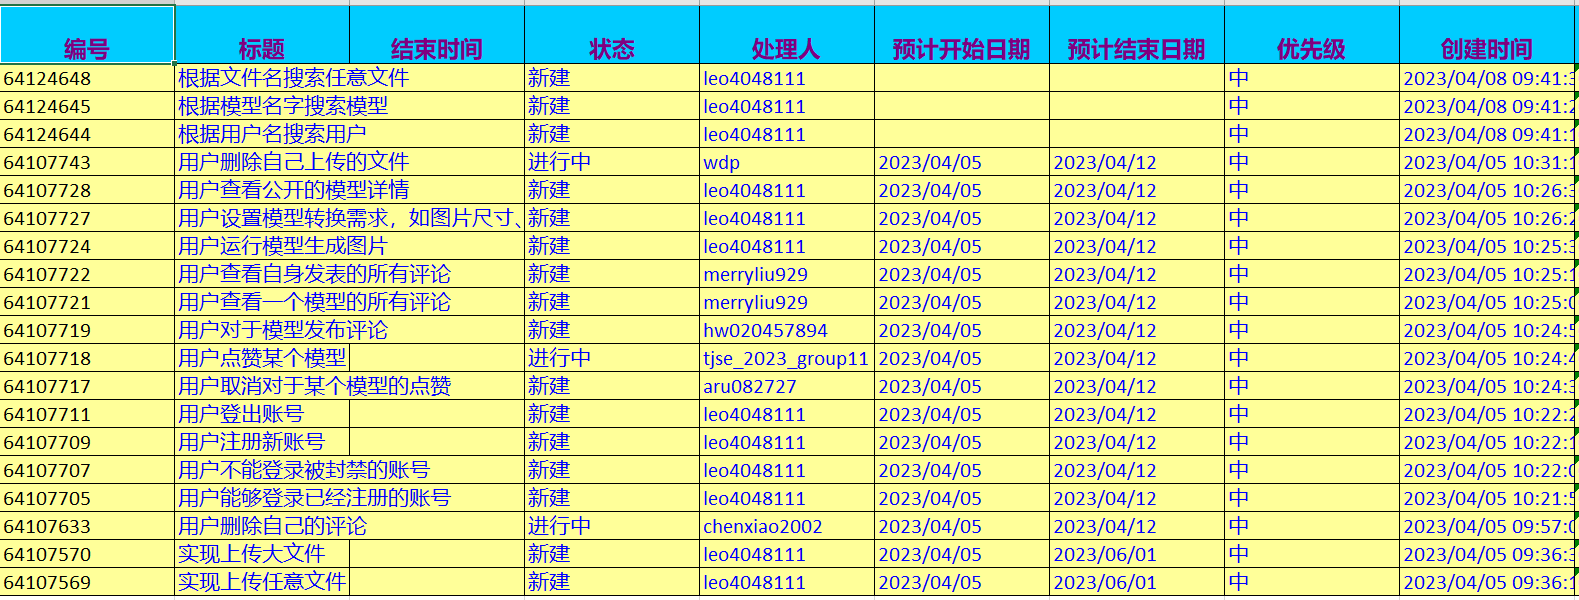
\includegraphics[width=\textwidth]{contents/figure/iteration1_stories.png}
    \end{figure}
\end{frame}

\section{第一次迭代开发成果展示}
\begin{frame}{用户注册新账号}
    \begin{itemize}
        \item 用户故事描述:作为一个新用户,我想要注册一个新账号,以便于使用网站的各种功能和服务。
        \item 接口责任人:李其桐
        \item 功能页面设计: //TODO
    \end{itemize}
\end{frame}

\begin{frame}{用户登录账号}
    \begin{itemize}
        \item 用户故事描述:作为一个已注册的用户,我想要登录我的账号,以便于使用网站的各种功能和服务。
        \item 接口责任人:李其桐
        \item 附加信息:如果用户已登录,并且没有进行登出操作,则关闭页面后再登录系统时应当能够自动验证会话并且跳转到主页。
        \item 功能页面设计: //TODO
    \end{itemize}
\end{frame}

\begin{frame}{用户查看自身上传的模型文件}
    \begin{itemize}
        \item 用户故事描述:作为一个AI绘画软件系统使用者,我想要查看我上传的模型文件,以便于管理我的作品和修改我的设计。
        \item 接口责任人:李其桐
        \item 功能页面设计: //TODO
    \end{itemize}
\end{frame}

\begin{frame}{用户删除自身上传的模型文件}
    \begin{itemize}
        \item 用户故事描述:作为一个AI绘画软件系统使用者,我想要删除我上传的模型文件,以便于清理我的空间、避免重复或错误的作品、或者更新迭代我的模型文件版本。
        \item 接口责任人:吴达鹏
        \item 功能页面设计:
    \end{itemize}
\end{frame}

\begin{frame}{用户删除自身上传的模型文件}
    \begin{figure}[H]
        \centering
        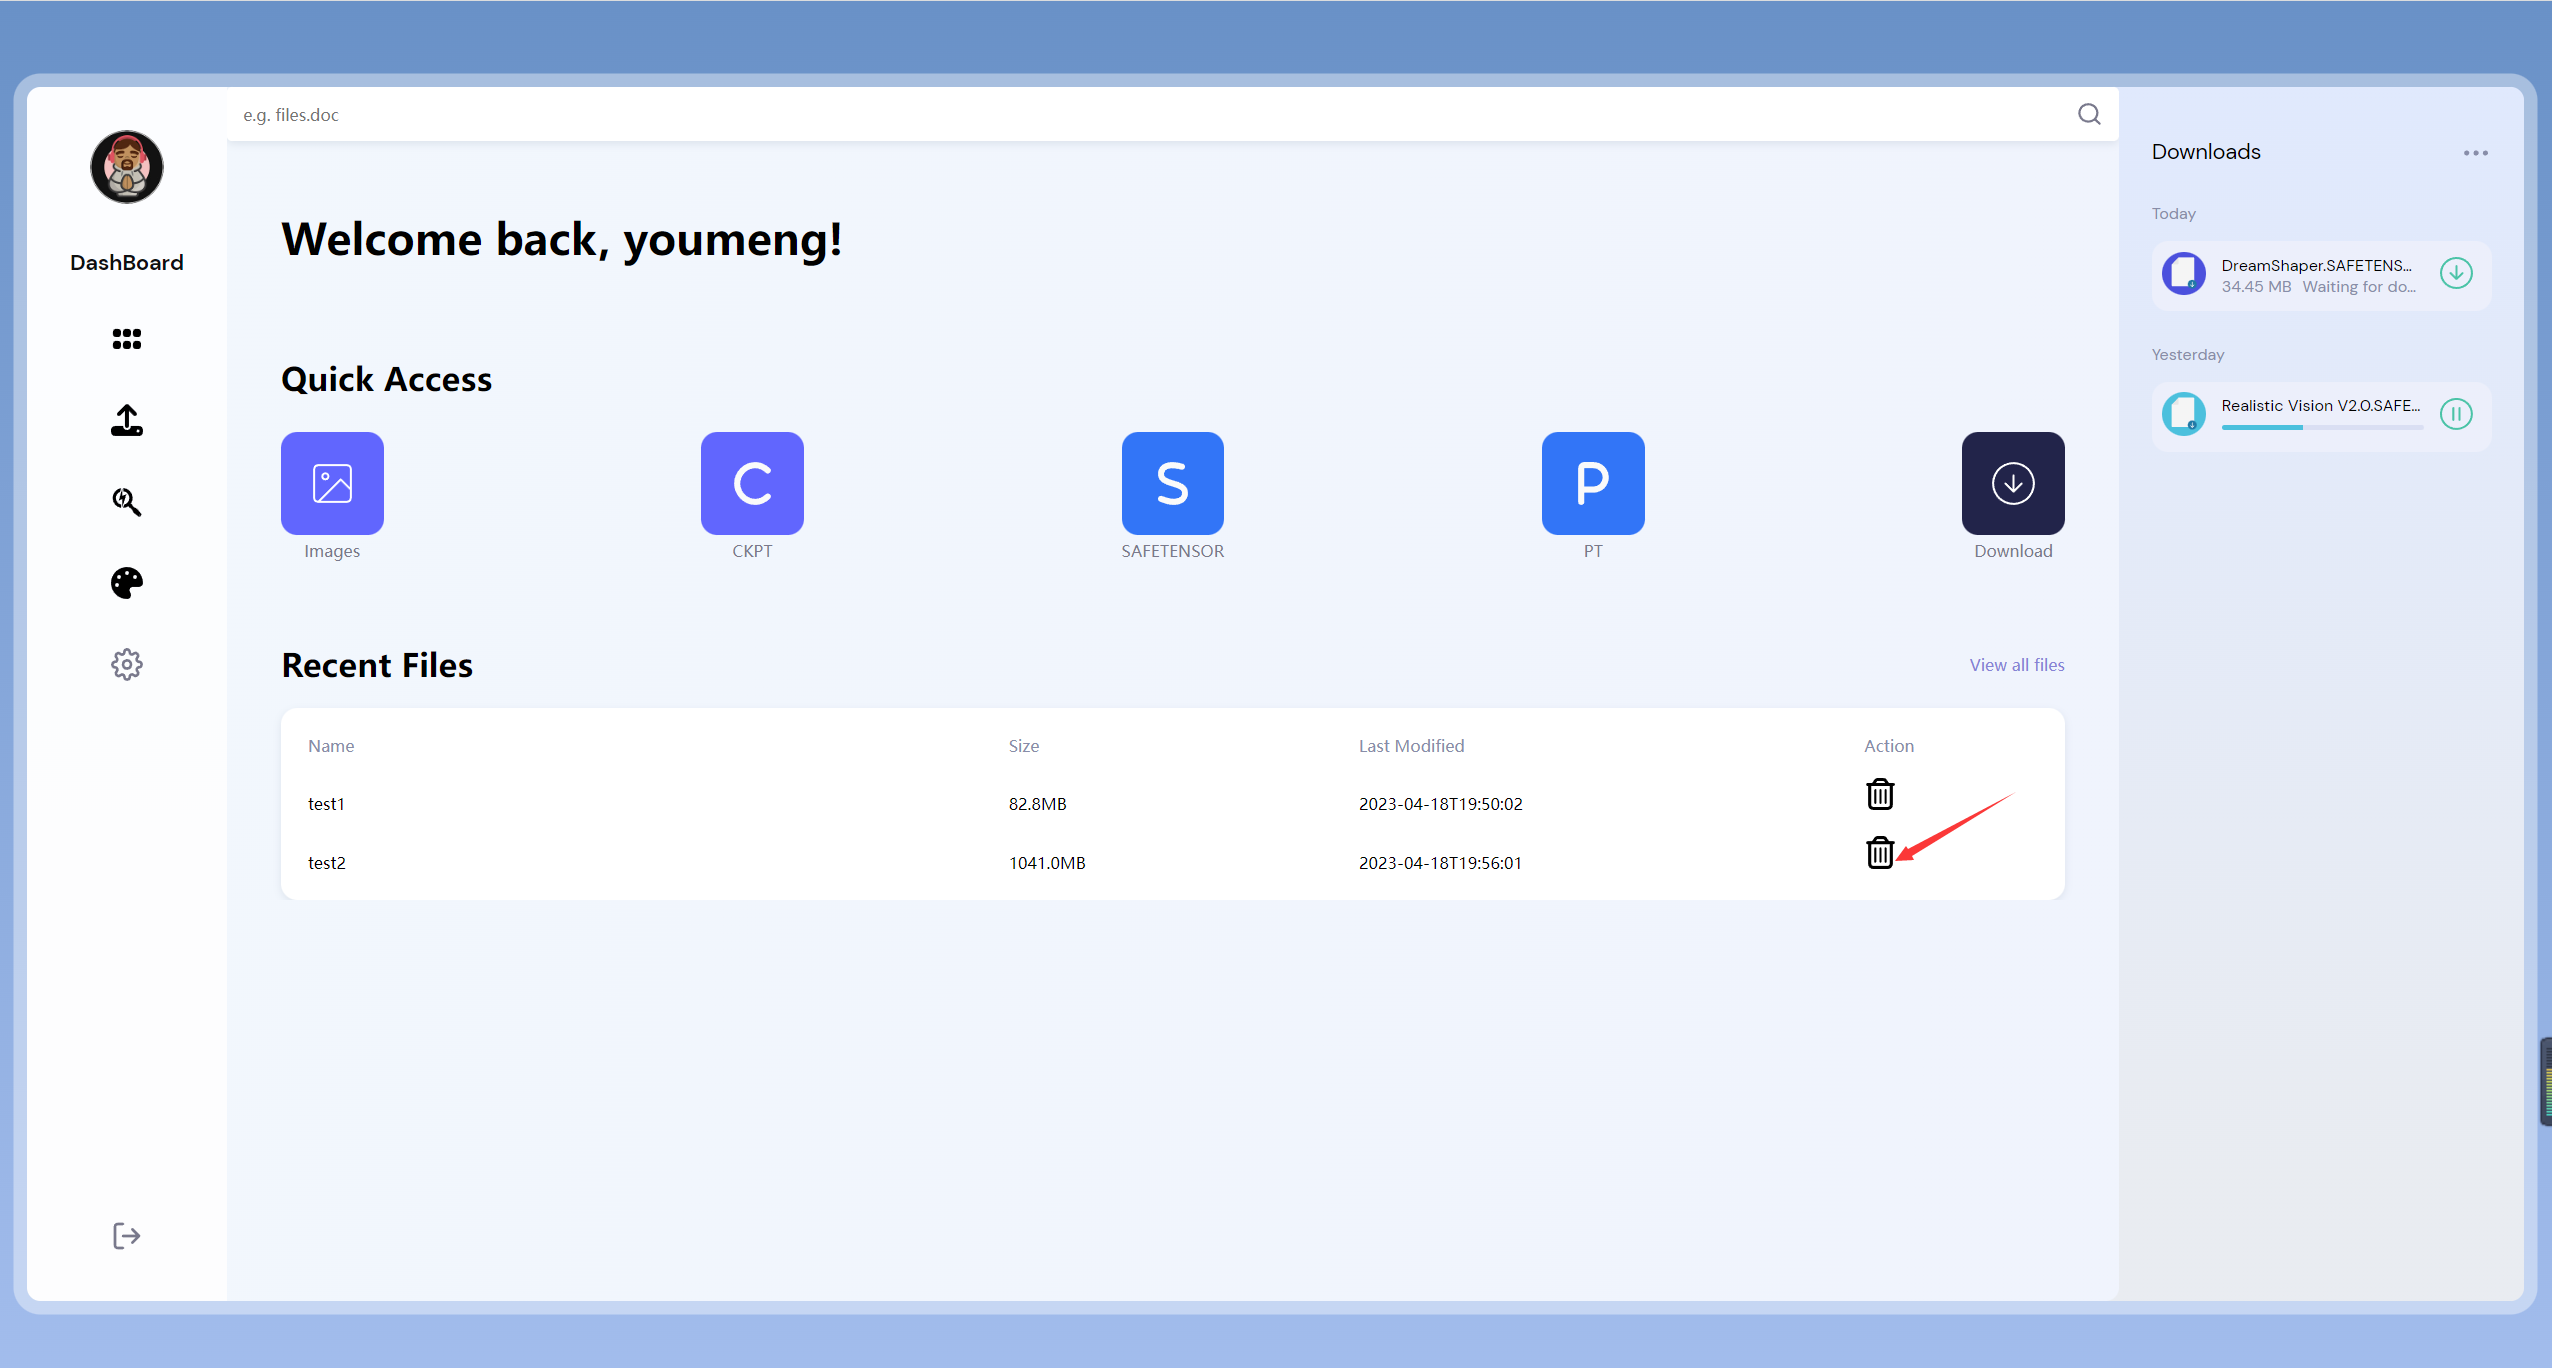
\includegraphics[width=\textwidth]{contents/figure/remove_click.jpg}
    \end{figure}
\end{frame}

\begin{frame}{用户删除自身上传的模型文件}
    \begin{figure}[H]
        \centering
        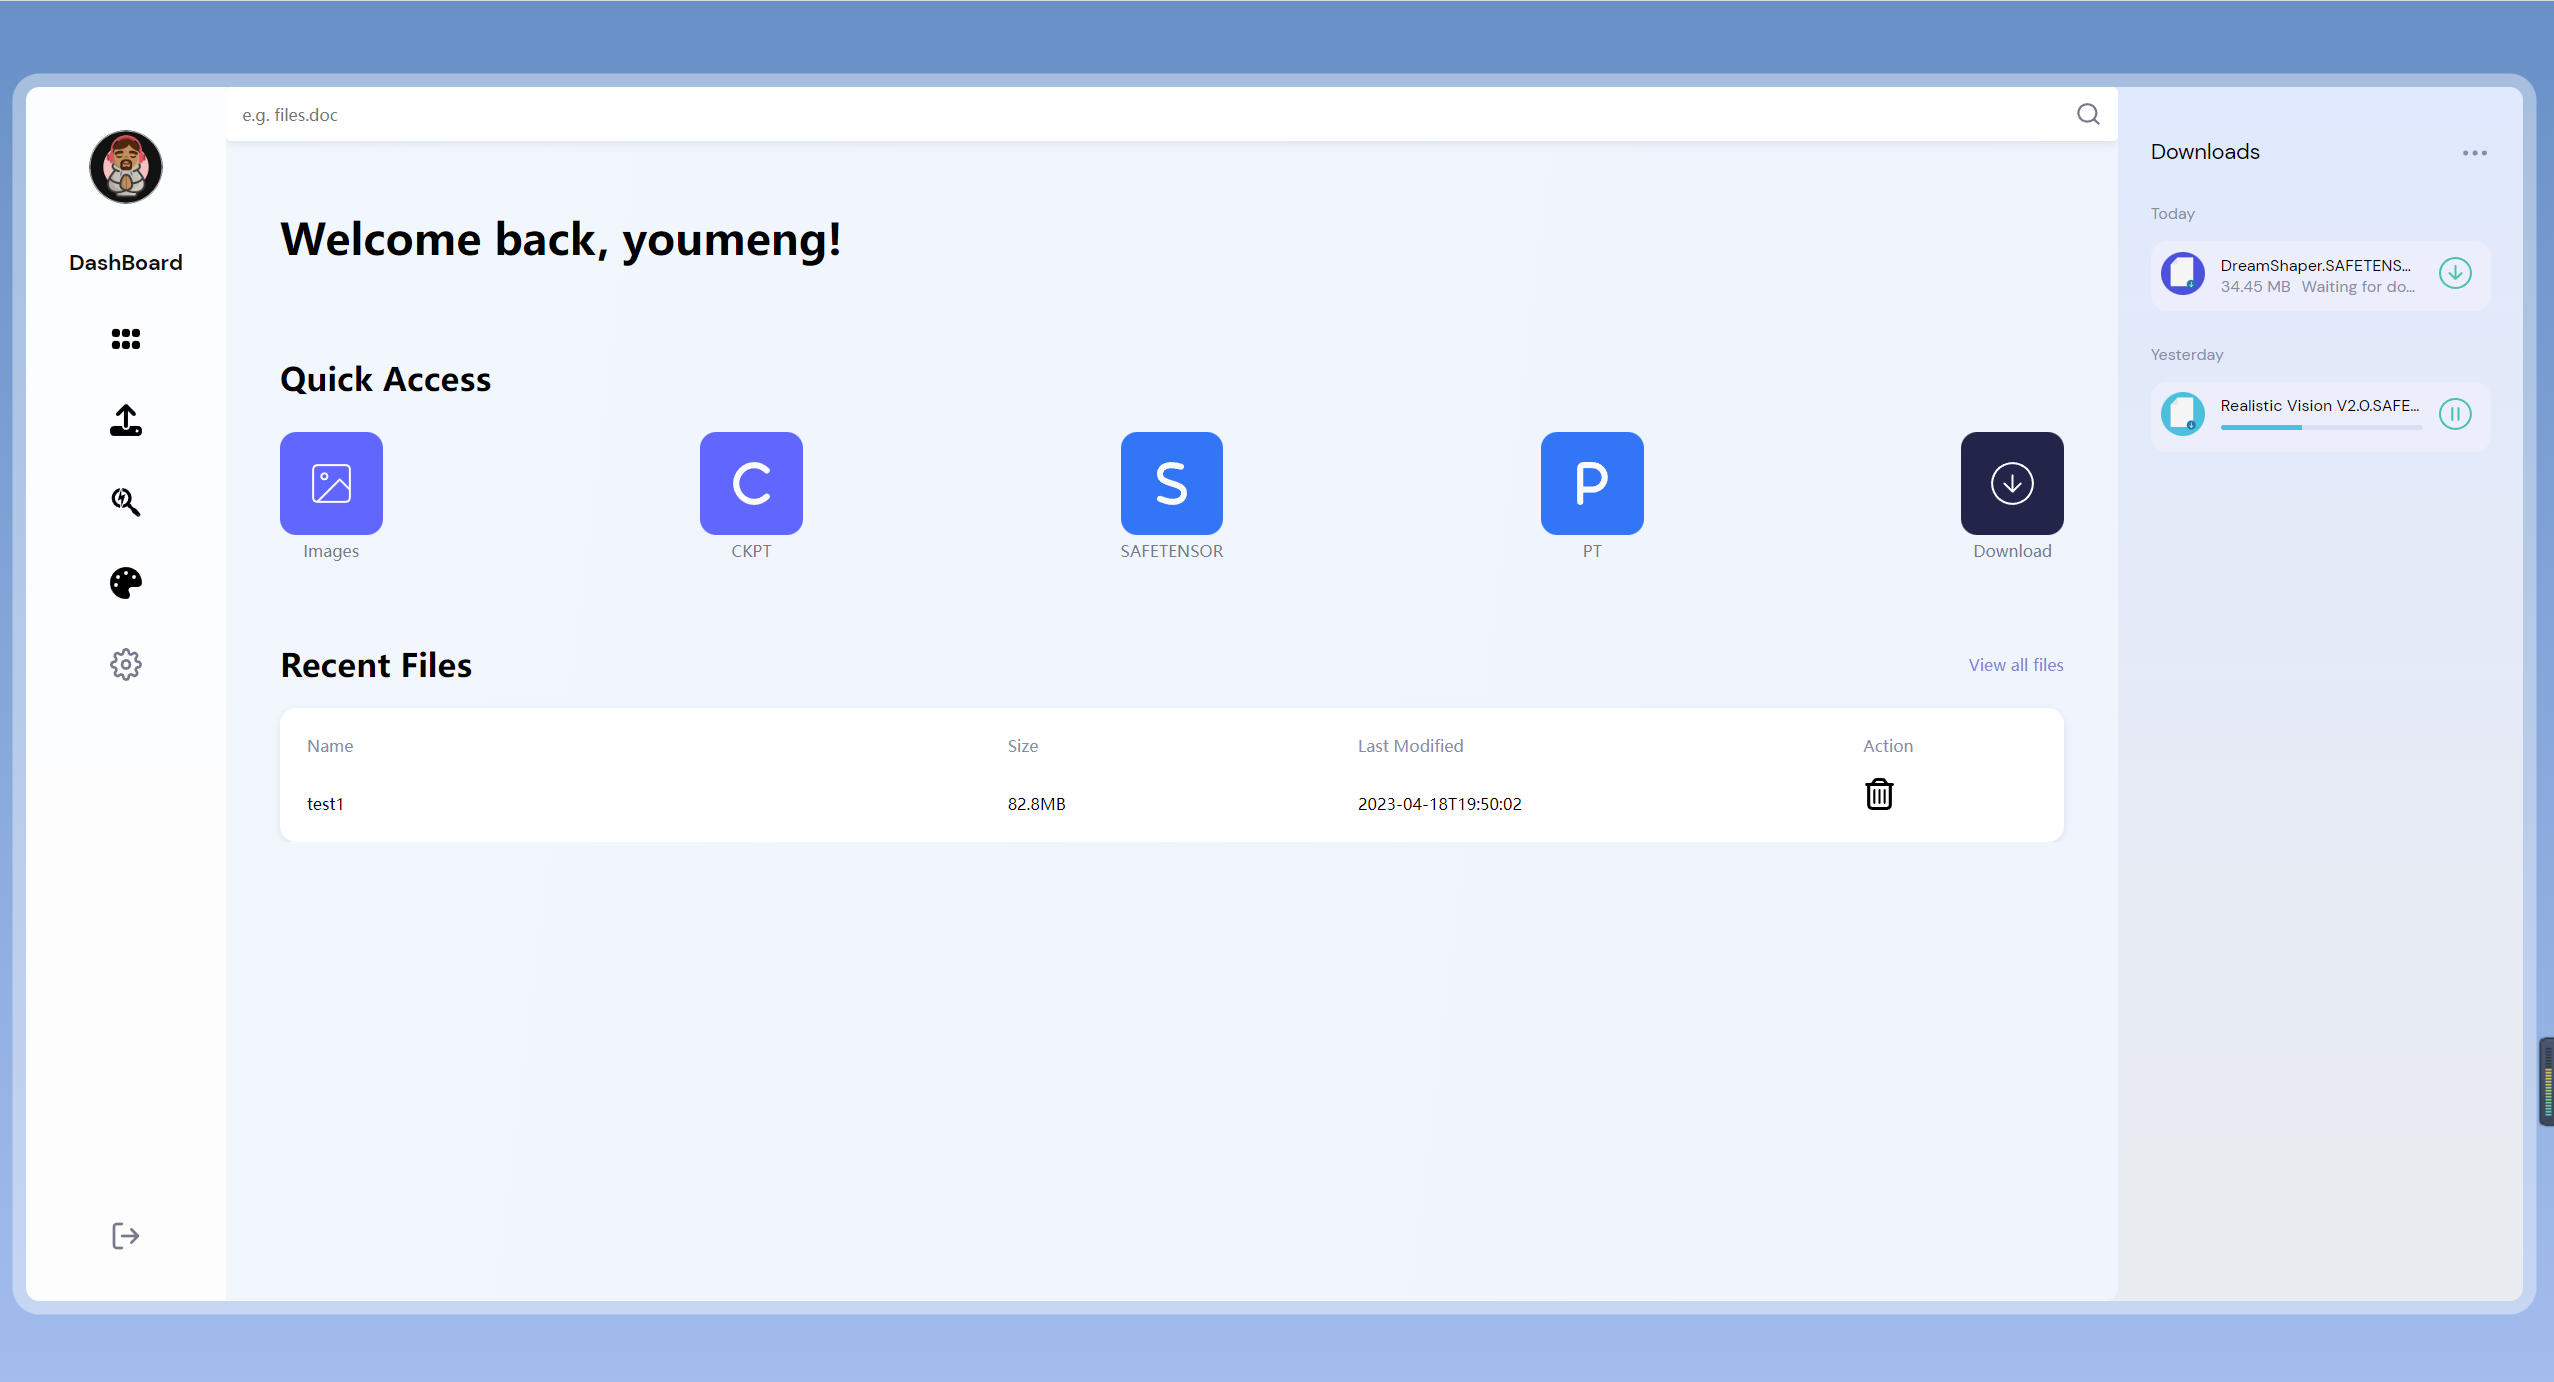
\includegraphics[width=\textwidth]{contents/figure/remove_result.jpg}
    \end{figure}
\end{frame}

\begin{frame}{根据模型名字搜索模型}
    \begin{itemize}
        \item 用户故事描述:作为一个模型使用者,我想要根据模型名字搜索模型,以便于快速找到我需要的绘图模型和相关信息。
        \item 接口责任人:李其桐
        \item 功能页面设计: //TODO
    \end{itemize}
\end{frame}

\begin{frame}{根据用户名搜索用户}
    \begin{itemize}
        \item 用户故事描述:作为一个模型使用者,我想要根据用户名搜索用户,以便于关注我喜欢的模型训练师和随时查看他们的作品并且获取他们的动态。
        \item 接口责任人:曾诗容
        \item 功能页面设计: //TODO
    \end{itemize}
\end{frame}

\begin{frame}{用户查看一个模型的所有评论}
    \begin{itemize}
        \item 用户故事描述:作为一个模型使用者,我想要查看一个模型的所有评论,以便于了解其他用户的反馈和建议。
        \item 接口责任人:刘昱彤
        \item 功能页面设计: //TODO
    \end{itemize}
\end{frame}

\begin{frame}{用户对于模型发表评论}
    \begin{itemize}
        \item 用户故事描述:作为一个模型使用者,我想要对一个模型发表评论,以便于表达我的意见和感受,以及和其他用户交流。
        \item 接口责任人:于采篱
        \item 功能页面设计: //TODO
    \end{itemize}
\end{frame}

\begin{frame}{用户删除已发表的评论}
    \begin{itemize}
        \item 用户故事描述:作为一个模型使用者,我想要删除我已发表的评论,以便于撤回我不想要的或错误的意见。
        \item 接口责任人:陈骁
        \item 功能页面设计: //TODO
    \end{itemize}
\end{frame}

\begin{frame}{用户点赞模型}
    \begin{itemize}
        \item 作为一个模型使用者,我想要点赞一个模型,以便于支持我喜欢的模型设计师和推荐优秀的模型给其他用户。
        \item 接口责任人:陈骁
        \item 功能页面设计: //TODO
    \end{itemize}
\end{frame}

\begin{frame}{用户取消对于一个模型的点赞}
    \begin{itemize}
        \item 用户故事描述:作为一个模型使用者,我想要取消对于一个模型的点赞,以便于更改我的喜好和评价。
        \item 接口责任人:林奕如
        \item 功能页面设计: //TODO
    \end{itemize}
\end{frame}

\begin{frame}{用户设置模型转换需求,如Prompt描述、图片尺寸、模型相关参数等等}
    \begin{itemize}
        \item 用户故事描述:作为一个模型使用者,我想要设置模型转换需求,如图片尺寸、模型相关参数等等,以便于根据我的具体需求和场景,定制化地使用模型。
        \item 接口责任人:陈骁
        \item 附加信息:转换需求设置应当能够加载网站中已有的模型文件,以便于用户能够快速地设置模型转换需求。
        \item 功能页面设计: //TODO
    \end{itemize}
\end{frame}

\begin{frame}{用户运行模型生成图片}
    \begin{itemize}
        \item 用户故事描述:作为一个模型使用者,我想要运行模型生成图片,以便于看到模型的效果和输出。
        \item 接口责任人:陈骁
        \item 功能页面设计: //TODO
    \end{itemize}
\end{frame}

\begin{frame}{用户登出}
    \begin{itemize}
        \item 用户故事描述:作为一个已登录的用户,我想要在我不需要使用软件系统的时候登出我的账号,以便于保护我的隐私和安全。
        \item 接口责任人:李其桐
        \item 功能页面设计: //TODO
    \end{itemize}
\end{frame}

% end
% \section{用户登录}
\begin{frame}
    \frametitle{用户登录用例图}
    \center
    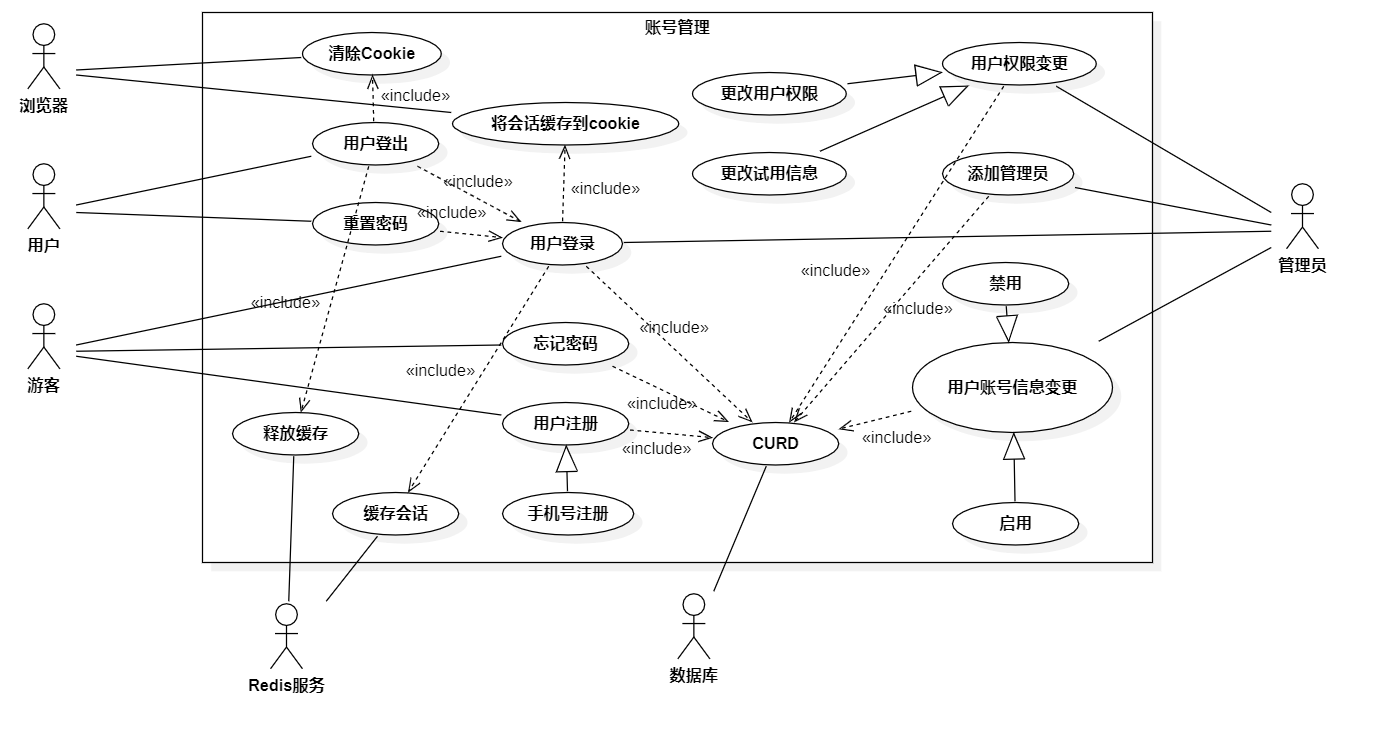
\includegraphics[width=4.5in]{contents/figure/login_usecase_diagram.png}
\end{frame}
\begin{frame}
    \frametitle{用户登录时序图}
    \center
    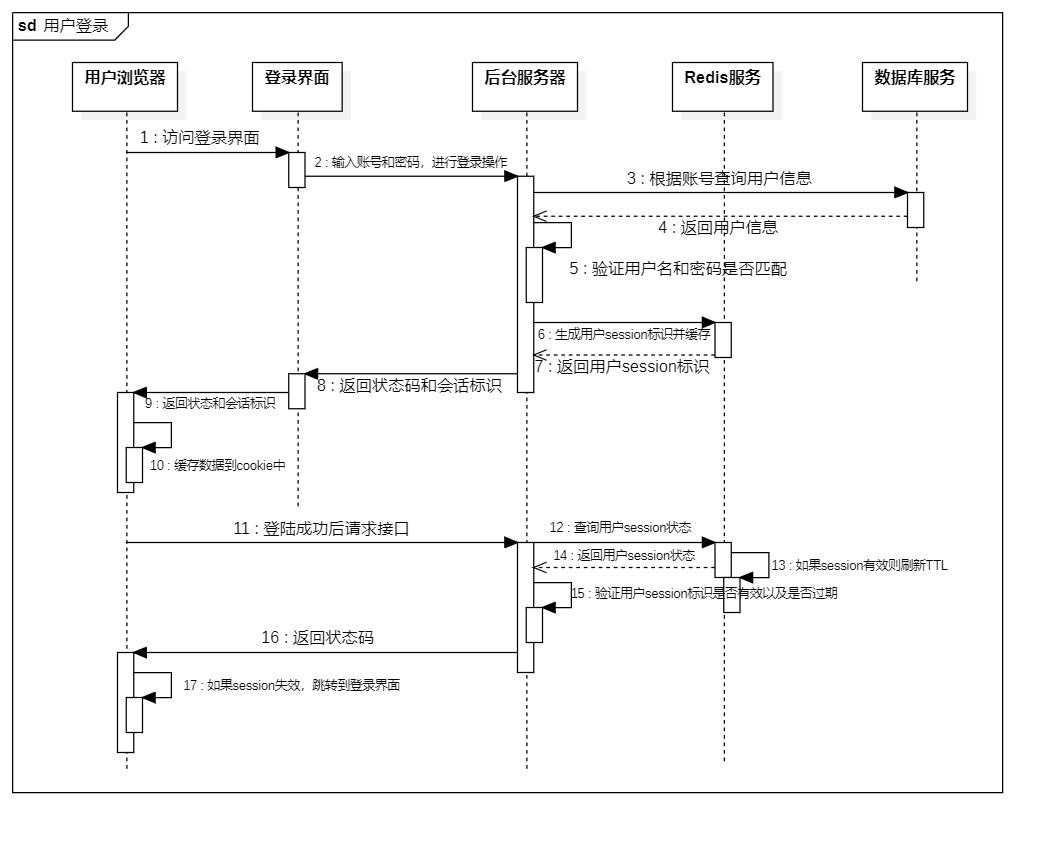
\includegraphics[width=3.8in]{contents/figure/login_sequence_diagram.png}
\end{frame}

% <<<<<<< Updated upstream
\section{文档编辑与PPT自动生成}
=======
\section{重点用例:文档编辑与PPT自动生成}
>>>>>>> Stashed changes
\begin{frame}
    \frametitle{文档编辑用例图}
    \center
    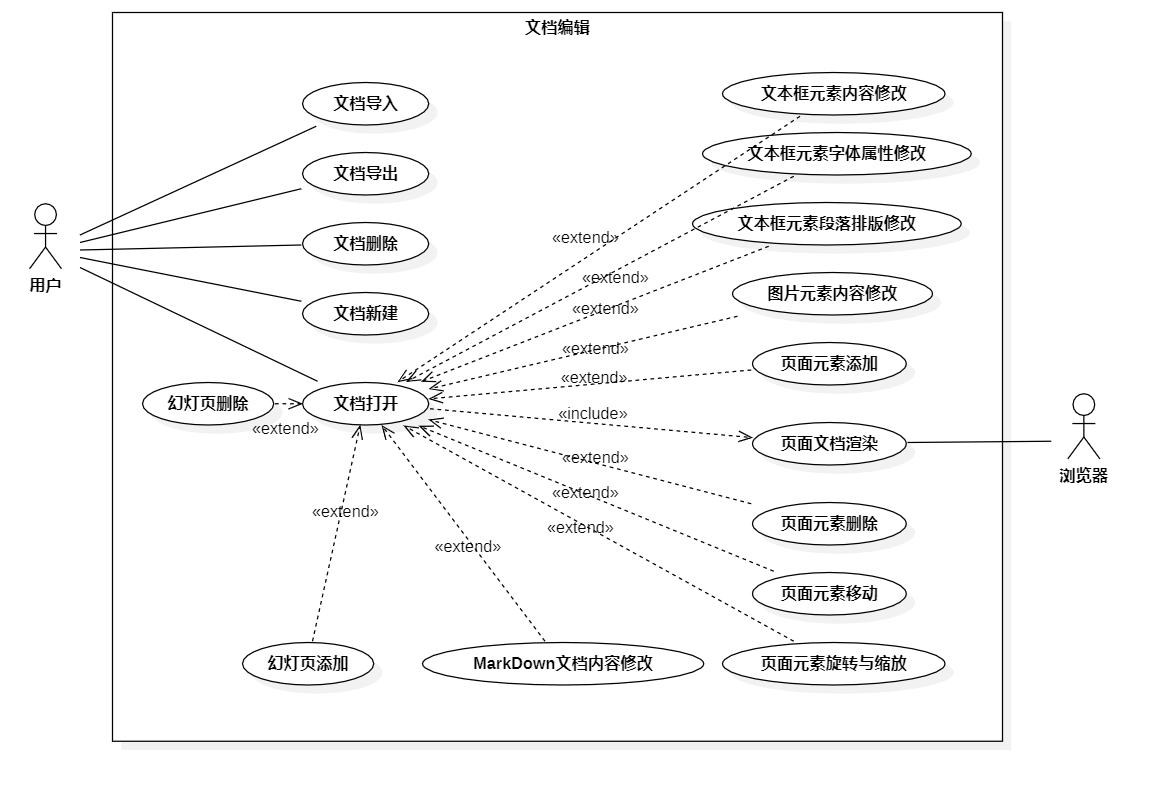
\includegraphics[width=4.0in]{contents/figure/ppt_generator_usercase_diagram.png}
\end{frame}
\begin{frame}
    \frametitle{PPT自动生成时序图}
    \center
    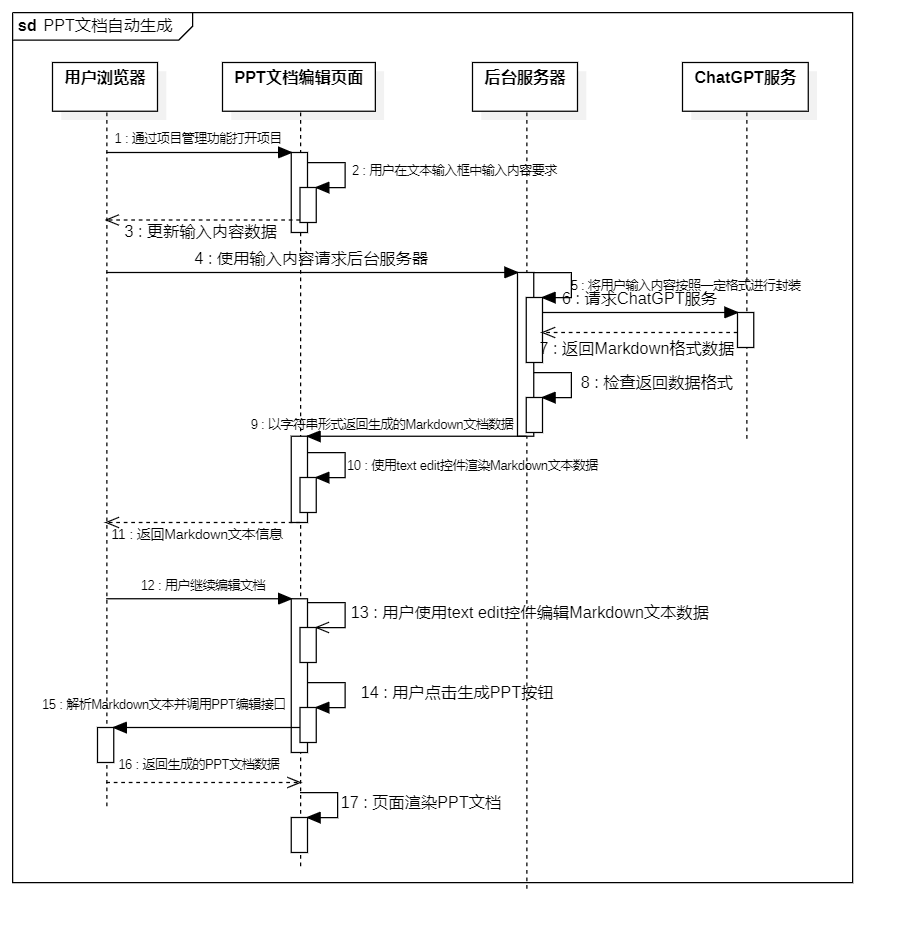
\includegraphics[width=2.8in]{contents/figure/ppt_generator_sequence_diagram.png}
\end{frame}
% <<<<<<< Updated upstream
\section{用户充值}
=======
\section{重点用例:用户充值}
>>>>>>> Stashed changes
\begin{frame}
    \frametitle{用户充值用例图}
    \center
    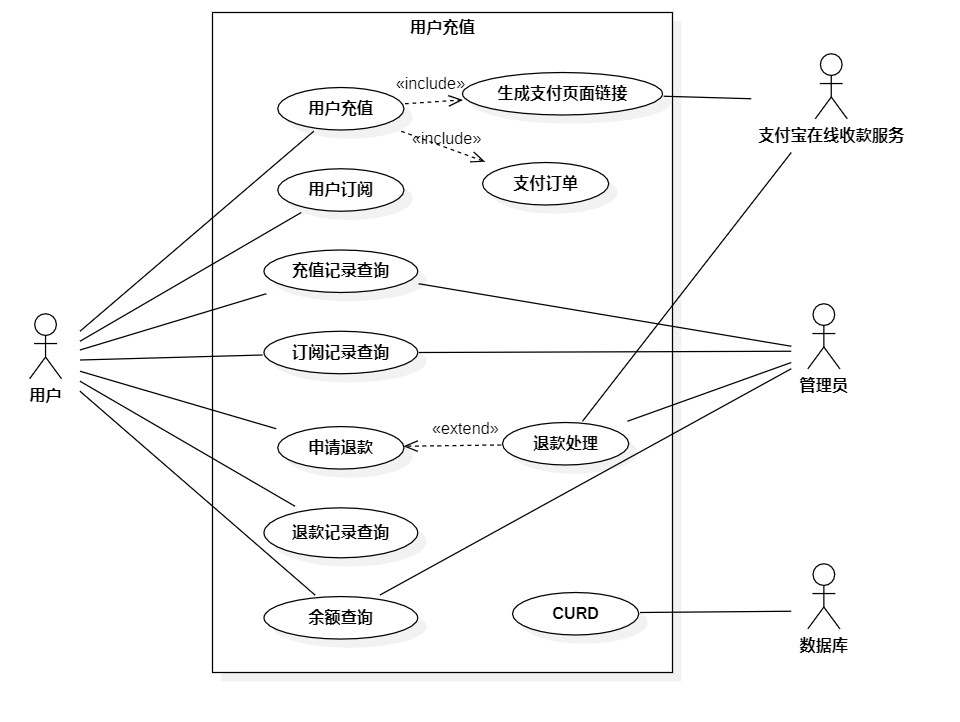
\includegraphics[scale=0.3]{contents/figure/recharge_usecase_diagram.png}
\end{frame}
\begin{frame}
    \frametitle{用户充值时序图}
    \center
    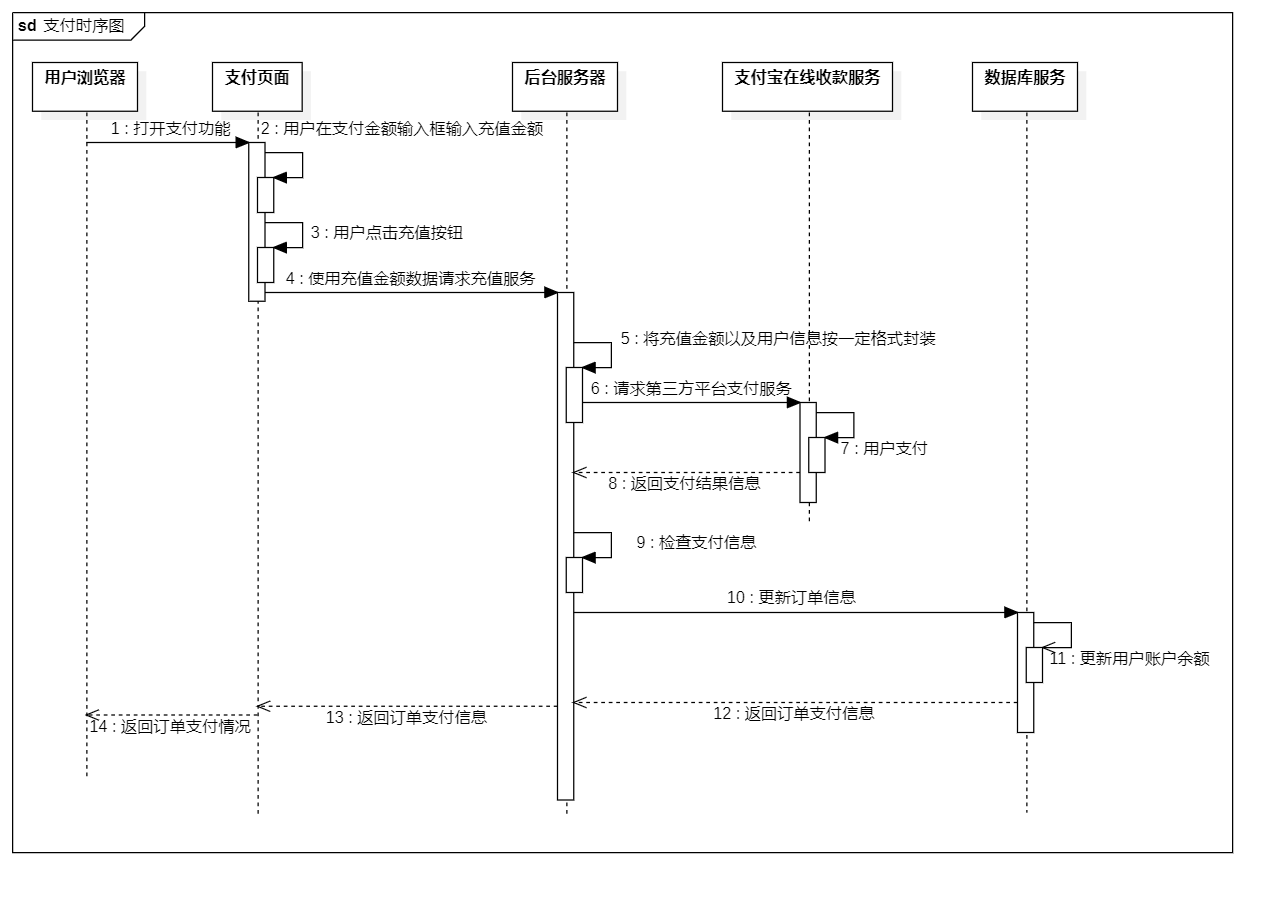
\includegraphics[width=4.2in]{contents/figure/recharge_sequence_diagram.png}
\end{frame}
% \section{非功能需求}
    \begin{frame}{质量属性}
        \begin{itemize}
            \item 可用性:保证高可用
            \item 可扩展性:功能扩展可仅通过添加文件、接口和修改外部界面实现
            \item 安全性:防范网络攻击
            \item 可靠性:可恢复、异常处理、不完全操作回滚
            \item 互操作性:导出文档能够直接在本地打开编辑
            \item 可维护性:用户操作记录、错误记录、网络访问记录等内容写入日志并落盘
            \item 可重用性:跨平台快速部署
            \item 可测试性:可进行单元测试、集成测试、系统测试、验收测试
        \end{itemize}
    \end{frame}

    \begin{frame}
        \frametitle{日志需求}
        \begin{enumerate}
            \item 后台应当实时维护能够让系统管理员查看的用户操作日志,其中记录包括用户行为、系统运行错误、网络访问记录和文件访问记录等主要内容。
            \item 用户行为中,登录、登出、注册、访问网页等主要行为需要被记录。
            \item 对存在可疑用户行为,比如对于登录频率超过20次/分钟、登录时连续输错密码超过10次,短时间类大量发起支付订单等行为的用户进行一定时间的禁用,并单独将行为记录在日志中。
            \item 日志数据应当持久化存储在磁盘上,并且支持快速记录检索和以文本形式导出并查看。
        \end{enumerate}
    \end{frame}

    \begin{frame}
        \frametitle{界面需求}
        \begin{enumerate}
            \item 软件系统界面元素应能够清晰呈现每个功能模块的用户交互逻辑,同时应避免过度设计,做到美观简洁。
            \item 软件系统界面的不同页面设计风格尽量统一。
        \end{enumerate}
    \end{frame}

    \begin{frame}
        \frametitle{服务器恢复需求}
        \begin{enumerate}
            \item 软件系统需要在例如物理机故障、掉电或者手动关闭服务时,能够尽可能保证关键数据,例如用户支付订单信息等的无差错和不丢失。
            \item 软件系统需要有定时备份机制,能够保证服务器上的数据可以定时备份,例如每周、每日或者每小时备份一次。 
            \item 软件系统需要有一个完整并且可操作性的恢复方案,可以表述在软件系统文档中,以能够在实际系统发生故障时,指导维护人员进行恢复操作。
        \end{enumerate}
    \end{frame}



% %% body.tex
%% Copyright 2022 skyleaworlder
%
% This work may be distributed and/or modified under the
% conditions of the LaTeX Project Public License, either version 1.3
% of this license or (at your option) any later version.
% The latest version of this license is in
%   http://www.latex-project.org/lppl.txt
% and version 1.3 or later is part of all distributions of LaTeX
% version 2003/12/01 or later.
%
% This work has the LPPL maintenance status "maintained".
%
% This Current Maintainer of this work is skyleaworlder.
%
% This work consists of all the *.tex and *.sty files in
%   https://github.com/TJ-CSCCG/Tongji-Beamer
\section{系统分析}
    % “图片文字并排” 示例
    \begin{frame}{内卷行为归因系统}
        \begin{columns}
            \column{.35\textwidth}
            \begin{figure}
                \centering 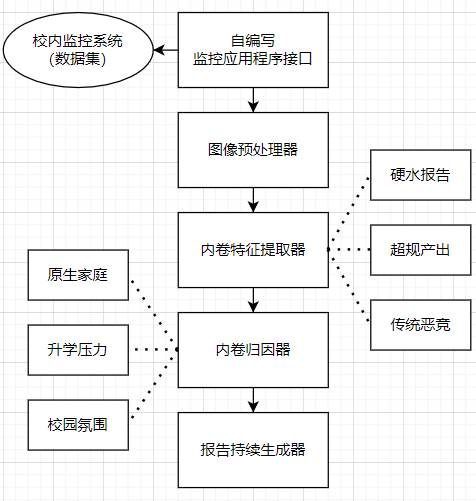
\includegraphics[width=2in]{contents/figure/factor-analyzer.png}
                \caption{归因系统架构}
                \label{fig:factor-analyzer}
            \end{figure}

            \column{.6\textwidth}
            \begin{itemize}
                \item 校内监控系统:接入校内系统,使用过往录像作为归因系统模型训练数据集。
                \item 特征提取器:项目提出了数十种内卷特征类型。提取器要求人工为部分数据集标记标签。
                \item 内卷归因器:阅读历史文献,得出数十种内卷成因,构建内卷特征到成因的映射函数。
                \item 报告持续生成器:开发该系统的报告生成器,提升用户体验。
            \end{itemize}
        \end{columns}
    \end{frame}

    % “图片文字垂直” 示例
    \begin{frame}{内卷识别器}
        \begin{figure}
            \centering
            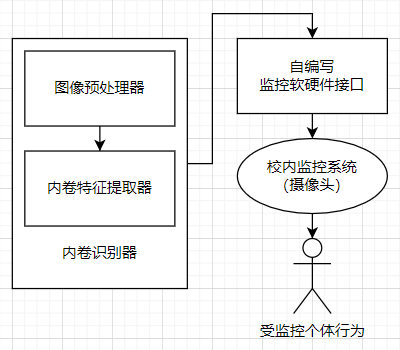
\includegraphics[width=.4\textwidth]{contents/figure/data-detector.png}
            \caption{识别器架构}
            \label{fig:data-detector}
        \end{figure}

        \begin{itemize}
            \item \small 复用归因系统中有关图像处理的 Phase,编写软硬件接口,对接校内监控系统终端设备。
            \item \small 识别器特征提取结果将上传至我校私有云上,方便监管与处理。
        \end{itemize}
    \end{frame}

    % “多图片文字混合” 示例
    \begin{frame}{内卷信息收集与行为防范系统}
        \begin{columns}
            \column{.4\textwidth}
            \begin{figure}
                \centering
                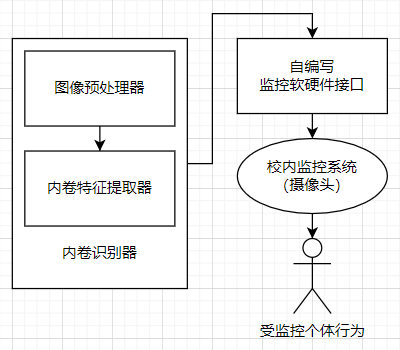
\includegraphics[width=\textwidth]{contents/figure/data-detector.png}
                \caption{识别器架构}
                \label{fig:data-detector-2}
            \end{figure}

            \column{.3\textwidth}
            \begin{figure}
                \centering
                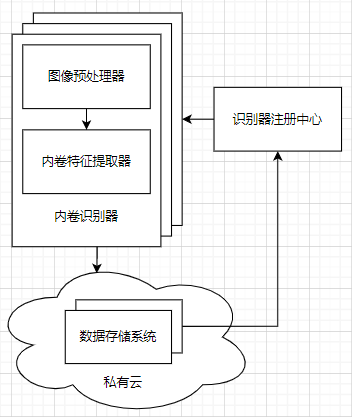
\includegraphics[width=\textwidth]{contents/figure/collector-part-1.png}
                \caption{信息收集系统}
                \label{fig:collector-part-1}
            \end{figure}

            \column{.3\textwidth}
            \begin{figure}
                \centering
                 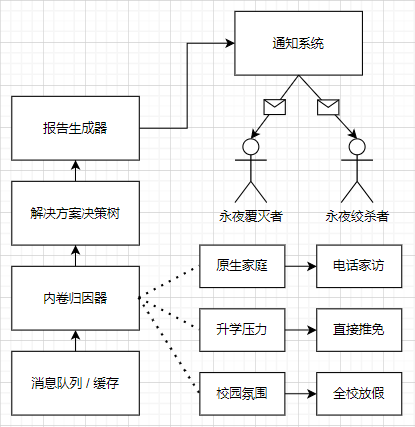
\includegraphics[width=\textwidth]{contents/figure/collector-part-2.png}
                \caption{行为防范系统}
                \label{fig:collector-part-2}
            \end{figure}
        \end{columns}

        \small 信息收集系统使用一个服务作为所有监控终端设备的 “注册中心”,提供鉴权、心跳检查等能力。行为规范系统复用了归因系统中有关因素分析的 Phase,以此作为决策树的判断基础。
    \end{frame}


\section{合理性分析}
    % “数学” 与 “公式” 示例
    \begin{frame}{专有名词释义}
        \begin{definition}[永夜势力]
            考虑一所高校,其中永夜村民的数量除以学生总数的值。
        \end{definition}
        \begin{theorem}[永夜定理]
            考虑一所高校,在不存在干涉的情况下,永夜势力在小于 1 前,恒呈指数型增长。
        \end{theorem}
        \begin{theorem}[永夜方程]
            考虑一所高校,人为干涉存在 x 的概率无效。x 是下列方程的解,其中 n 为全校学生总数。
        \end{theorem}

        \begin{equation}
            \begin{vmatrix}
            \begin{bmatrix}
                    x & \Phi(\pi) \\
                    \sum_{i = 1}^n xi & \exp(xi)
            \end{bmatrix}
            \begin{bmatrix}
                    1 & \cdots & n \\
                    x\Phi(e) & \cdots & x\Phi^n(e^n)
            \end{bmatrix}
            \end{vmatrix} = \dfrac{\pi}{x}
        \end{equation}
    \end{frame}

    % “简单公式” 示例
    \begin{frame}{负载分析}
        系统在设计时进行了计算下沉,分离图像处理的多个步骤,实现计算的高效性。

        假设 $id \in [1850001, 1859999]$,识别器与分析器共有 $m$ 个机器,第 $i$ 个机器负责 $[1850001 + i \times \frac{9999}{m}, 1859999 + (i + 1) \times \frac{9999}{100}]$ 个单位。

        识别层机器会发送分析层机器需要的特定记录到存储中。存储中每个节点大小为 16 KB,由于一条记录占据 4 00B 的空间,有:

        $$
        Node = \dfrac{16 \times 1024 B}{400 B} \approx 16
        $$

        假设 $t$ 为一次操作所花费的时间,设单表大小为 $M$。在不进行计算分离时,消耗的时间 $T = Mt$。但在分离过后,全过程时间为:

        $$
        T' = \dfrac{M}{m} + \dfrac{9999}{m} \times t < Mt, \quad if\ m > \dfrac{1}{t} + \dfrac{9999}{M}
        $$
    \end{frame}


\section{组件设计}
    % “表格” 示例
    \begin{frame}{决策系统设计}
        \begin{table}[]
            \centering
            \begin{tabular}{c|c|c}
            \textbf{运行时间} & \textbf{实验组} & \textbf{对照组(单位 1)} \\
            \hline
                设计模式使用 vs. 不使用 & 1.1 & 1 \\
                Julia vs. Python & 0.7 & 1 \\
                负载均衡集群 vs. 单机 & 0.5 & 1 \\
                集群分布式缓存 vs. 无缓存 & 0.8 & 1 \\
            \end{tabular}
            \caption{各技术对决策系统的影响}
            \label{tab:tech-strategy}
        \end{table}

        \begin{columns}
            \small
            \column{.5\textwidth}
            \begin{itemize}
                \item 使用 Strategy 设计模式。
                \item 使用 Julia 高效计算矩阵乘法。
                \item 对归因系统暴露幂等性 API,使用计算集群增强计算能力。
            \end{itemize}

            \column{.5\textwidth}
            \begin{itemize}
                \item 采用负载均衡,平衡集群中各处理机的负载。
                \item 采用分布式缓存技术,加快集群整体对高频特殊输入的反应。
            \end{itemize}
        \end{columns}
    \end{frame}

    % “引用” 示例
    \begin{frame}{通知系统设计}
        著名哲人 skyleaworlder 有言:“内卷是可以被扼杀在摇篮中的。"\cite{involution} 只要在检测到疑似内卷行为后做到及时响应,由专业技术人员发起干涉,就有很相当概率阻止永夜势力的扩张。

        通知系统需要具备以下几个方面特性:
        \begin{enumerate}
            \item 即时性。内卷极易滋生壮大,通知专业技术人员的时间应该尽可能短。
            \item 高可用性。内卷行为来势汹汹,需要保证通知系统推送功能在高并发环境下的高可用性。
        \end{enumerate}

        自然卷说过:“内卷是凡人在挣扎中写下的血与泪的史诗。"\cite{undergrads_inv} 这份 “扭曲的美” 不应存于世间。
    \end{frame}

%% summary.tex
%% Copyright 2022 skyleaworlder
%
% This work may be distributed and/or modified under the
% conditions of the LaTeX Project Public License, either version 1.3
% of this license or (at your option) any later version.
% The latest version of this license is in
%   http://www.latex-project.org/lppl.txt
% and version 1.3 or later is part of all distributions of LaTeX
% version 2003/12/01 or later.
%
% This work has the LPPL maintenance status "maintained".
%
% This Current Maintainer of this work is skyleaworlder.
%
% This work consists of all the *.tex and *.sty files in
%   https://github.com/TJ-CSCCG/Tongji-Beamer
\section{总结}
    \begin{frame}{总结}
        “永夜星弓” 系统已在我校试运行 2 个月。试运行期间,上报内卷行为 300'000 起,成功制止 280'000 次轻微内卷行为、10'000 次中等内卷行为以及 10'000 次重度内卷行为。

        \begin{center}
            感谢在毕业设计实现过程中提供指导的老师们!

            感谢在这百余天中一直陪伴我的家人和同学们!

            感谢这个美丽的世界给了我从大学毕业的机会!
        \end{center}

        \begin{center}
            谢谢各位!请多多指教!
        \end{center}
    \end{frame}

% \begin{frame}{参考文献}
%     \printbibliography
% \end{frame}

\end{document}
